\documentclass{ExcelAtFIT}
%\documentclass[czech]{ExcelAtFIT} % when writing in CZECH
%\documentclass[slovak]{ExcelAtFIT} % when writing in SLOVAK


%--------------------------------------------------------
%--------------------------------------------------------
%	REVIEW vs. FINAL VERSION
%--------------------------------------------------------

%   LEAVE this line commented out for the REVIEW VERSIONS
%   UNCOMMENT this line to get the FINAL VERSION
\ExcelFinalCopy


%--------------------------------------------------------
%--------------------------------------------------------
%	PDF CUSTOMIZATION
%--------------------------------------------------------

\hypersetup{
	pdftitle={Paper Title},
	pdfauthor={Author},
	pdfkeywords={Keyword1, Keyword2, Keyword3}
}

%--------------------------------------------------------
%--------------------------------------------------------
%	ARTICLE INFORMATION
%--------------------------------------------------------

\ExcelYear{2018}

\PaperTitle{Machine Translation Using Artificial Neural Networks}

\Authors{Jonáš Holcner*}
\affiliation{*%
  \href{mailto:xholcn01@stud.fit.vutbr.cz}{xholcn01@stud.fit.vutbr.cz},
  \textit{Faculty of Information Technology, Brno University of Technology}}

\Keywords{neural machine translation --- NMT --- recurrent neural networks --- RNN ---
LSTM --- encoder-decoder architecture --- sequence to sequence --- seq2seq ---
keras --- moses --- BLEU}

\Supplementary{\href{https://github.com/jojkos/neural-machine-translation}{Downloadable Library}}


%--------------------------------------------------------
%--------------------------------------------------------
%	ABSTRACT and TEASER
%--------------------------------------------------------

\Abstract{
The aim of this work is to develop a neural machine translation system (NMT). This is a machine translation system based on neural networks. Specifically, the system is based on an encoder-decoder architecture, created with recurrent neural networks enabling sequence-to-sequence translation. The system is built with Keras and Tensorflow libraries and is tested against Moses statistical machine translation tool. This work does not bring any specific new state-of-the-art model but shows an insight into the topic. The result is an open source python library provided for public use.
}

\Teaser{
	%\TeaserImage{teaser1.pdf}
	%\TeaserImage{teaser2.pdf}
	%\TeaserImage{teaser3.pdf}
    
\includegraphics[width=1\linewidth]{excelTeaser.pdf}
}

%--------------------------------------------------------

\begin{document}

\startdocument

%--------------------------------------------------------
%	ARTICLE CONTENTS
%--------------------------------------------------------

\section{Introduction}
In the recent years, there is a significant increase in usage of a machine learning and an artificial intelligence. This is because, the capacity and performance of computers caught up with the available amount of data that is being produced every day, as to build and train large enough machine learning models. Nowadays, neural networks are widely capable of recognizing images, transcribing spoken language and most interestingly for this paper, they are quite capable in translating sequences from a one language to another.

The biggest advantage of the modern neural machine translation (\emph{NMT}) approach is that it does not have some of the problems the traditional machine translation systems had. Instead of translating only parts of sentences or phrases, NMT has the ability to learn and translate directly whole sequences in end-to-end fashion.

The goal of this work is to develop and try out such system and provide an out of the box usable library. The solution proposed in this paper makes use of the encoder-decoder architecture.

The result is python package \emph{nmt} built with Keras and Tensorflow machine learning libraries. Experiments with test datasets were conducted using this package, evaluated with the standard BLEU score. Results were compared with the system produced by the Moses \cite{Moses} statistical machine tool.


\section{Previous Works}
The first idea of the recurrent neural networks (RNN) comes from the nineties \cite{rnn}. The vanilla RNN, however, had a problem with long term dependencies because of the vanishing and exploding gradients \cite{gradientProblems}.

Thus came improved variants of the RNN -- long short term memory (LSTM) \cite{LSTM, forgetLSTM} and its simpler version, gated recurrent unit (GRU) \cite{GRU}. These units have a memory, that stores and changes information in it over time, enabling the network to remember long term dependencies.

Works \cite{neuralLanguageModels, neuralLanguageModels2, mikolovphd} showed that then state-of-the-art language models were built using recurrent neural networks. This layed a foundation for the neural machine translation as language models are the vital part. The advantage of neural language model is that it learns embeddings (Figure \ref{figure:oneHotAndEmbedding}) in a continuous space for the words, which provides the model with more context it can learn from.

\begin{figure}[h!]
    \begin{center}
        $V$ = $[$farmer, cow, steak, eats, \dots$]$ \\ \vspace{5mm}
        $
        oneHot_{steak}=
        \begin{bmatrix}
            0 \\
            0 \\
            1 \\
            0 \\
            \vdots \\
        \end{bmatrix}
        $ \\ \vspace{5mm}
        $
        wordEmbedding_{steak}=
        \begin{bmatrix}
            x_0 \\
            x_1 \\
            $\vdots$ \\
            x_{300} \\
        \end{bmatrix}
        $
    \end{center}
	\caption{Difference between common representation and word embeddings representation of words from vocabulary $V$. Common one-hot sparse vector represent the word with 1 on the position in the vector that corresponds with the index of the word in the vocabulary. Word embedding dense vector on the other hand represents the word with a for example vector of size 300, which holds some semantic value of the word and thus can be better utilized by the neural network.}
	\label{figure:oneHotAndEmbedding}
\end{figure}

Different variants of learning the word embbeddings are shown here \cite{word2vec,kingQueen,glove,fasttext}. Pre-trained word  embeddings, for example on some very large data set, can be used to boost the performance of a NMT system, which would have to otherwise learn those embeddings by itself.

The encoder-decoder architecture was proposed in \cite{encoderDecoder} and was used for rescoring hypotheses produced by a phrase-based system with a successful improvement. Sutskever et al. \cite{seq2seq} then showed how to use the encoder-decoder architecture for direct sequence-to-sequence translation and comes with the best results at the time. Furthermore, it was found that reversing order of the words in all source sentences (reverse encoder), improves models performance, by introducing short term dependencies between the source and the target sentence.

Upon this builds the work \cite{attention} which shows even better results with the bi-directional encoder which is an encoder that process sequences in both forward and reverse order. What is even more important, they address the problem of the encoder-decoder approach, where the meaning of the translated sentence is captured in a fixed-length vector and that can be problematic for translating long sentences. The proposed remedy is so called \emph{attention} mechanism which lets the model, at the time of decoding, look at the most important words from the source sentence for the currently translated word, resulting in even better performance.

As translation is an open-vocabulary problem, the NMT systems have to somehow handle the words not present at the time of the training. This was typically done by using out-of-vocabulary tokens and by using very large vocabularies, which causes the models to be very memory and performance demanding. A solution for this can be sub-word units \cite{mikolovSubwords, subwords}, that are shown to be more efficient, help with rare and unknown words and improve the results.

Current state-of-the-art results \cite{googleBridgingGap,googleAttention}, uses all of the techniques described, showing that they can be successfully applied on large production data sets.

Johnson et al. \cite{googleMultiLingual} shows, that with no changes to the model architecture, one model can be used to learn to translate between many languages, even to produce translations between languages that it was not explicitly trained on (zero-shot translations).

\section{Seq2seq translation with encoder-decoder architecture}
Sequence-to-sequence (\textbf{seq2seq}) means that the process of translating takes one whole sentence at the input, in a source language, and its meaning translates into a sequence in a target language. This can be better in contrast to other methods like word-based translation or phrase-based translation as in seq2seq the whole meaning of the source sequence is translated at once and can keep the precise meaning. Seq2seq is modeling probability of a target sentence based on a source sentence as shown in Figure \ref{fig:seqProbability}.

The neural network architecture, used for this kind of modeling, is \textbf{encoder-decoder}. Both the encoder and the decoder are recurrent neural network (Figure \ref{fig:rnn}), usually one or more layers of LSTM or GRU.

\begin{figure}[h!]
    \begin{center}
        \setlength{\fboxsep}{8pt}
        \fbox{$W_{in}$ = ``Ahoj světe"}
        $\Longrightarrow$
        \fbox{$W_{out}$ = ``Hello world"}
    \end{center}
	\caption{Seq2seq models a probability $P(W_{out}|W_{in})$. Meaning that the model learns to predict a sentence $W_{out}$ based on a sentence $W_{in}$.}
	\label{fig:seqProbability}
\end{figure}

\begin{figure}[h!]\centering
  \centering
  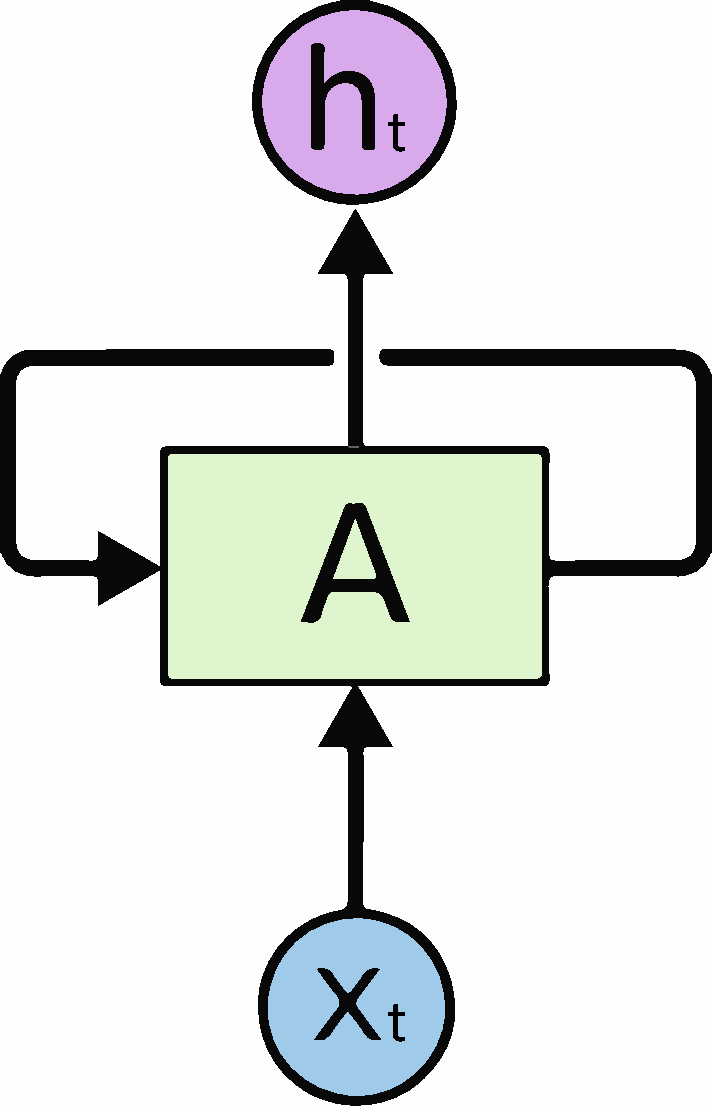
\includegraphics[width=0.4\linewidth]{RNN-rolled}
  \caption{RNN are neural networks with loops. They process sequence of data and an output $h_t$ from each time step $t$ is fed as an input to the time step $t+1$. The image is taken from \cite{understandingLSTM}.}
  \label{fig:rnn}
\end{figure}


The encoder takes embeddings of the input tokens (words or subwords) and processes the input sequence in a source language into a fixed-length vector, the so called ``thought" vector -- it captures the essence of the given sentence.

The hidden state of a decoder is initialized with this output from an encoder. The decoding process is started with a start token, which is given to the decoder as the first input. The decoder then generates a sequence in the target language until it reaches an end token that tells it to stop. There is a difference between the time when model is being trained and between the time when it is used to predict sequences. In the training time, the decoder is fed the correct, expected output. This is called ``teacher forcing" \cite{teacherForcing}. In the inference time, the decoder is fed its own output the each time step. The Figure \ref{fig:seq2seq} shows the encoder-decoder architecture.

\begin{figure*}[h!]\centering % Using \begin{figure*} makes the figure take up the entire width of the page
  \centering
  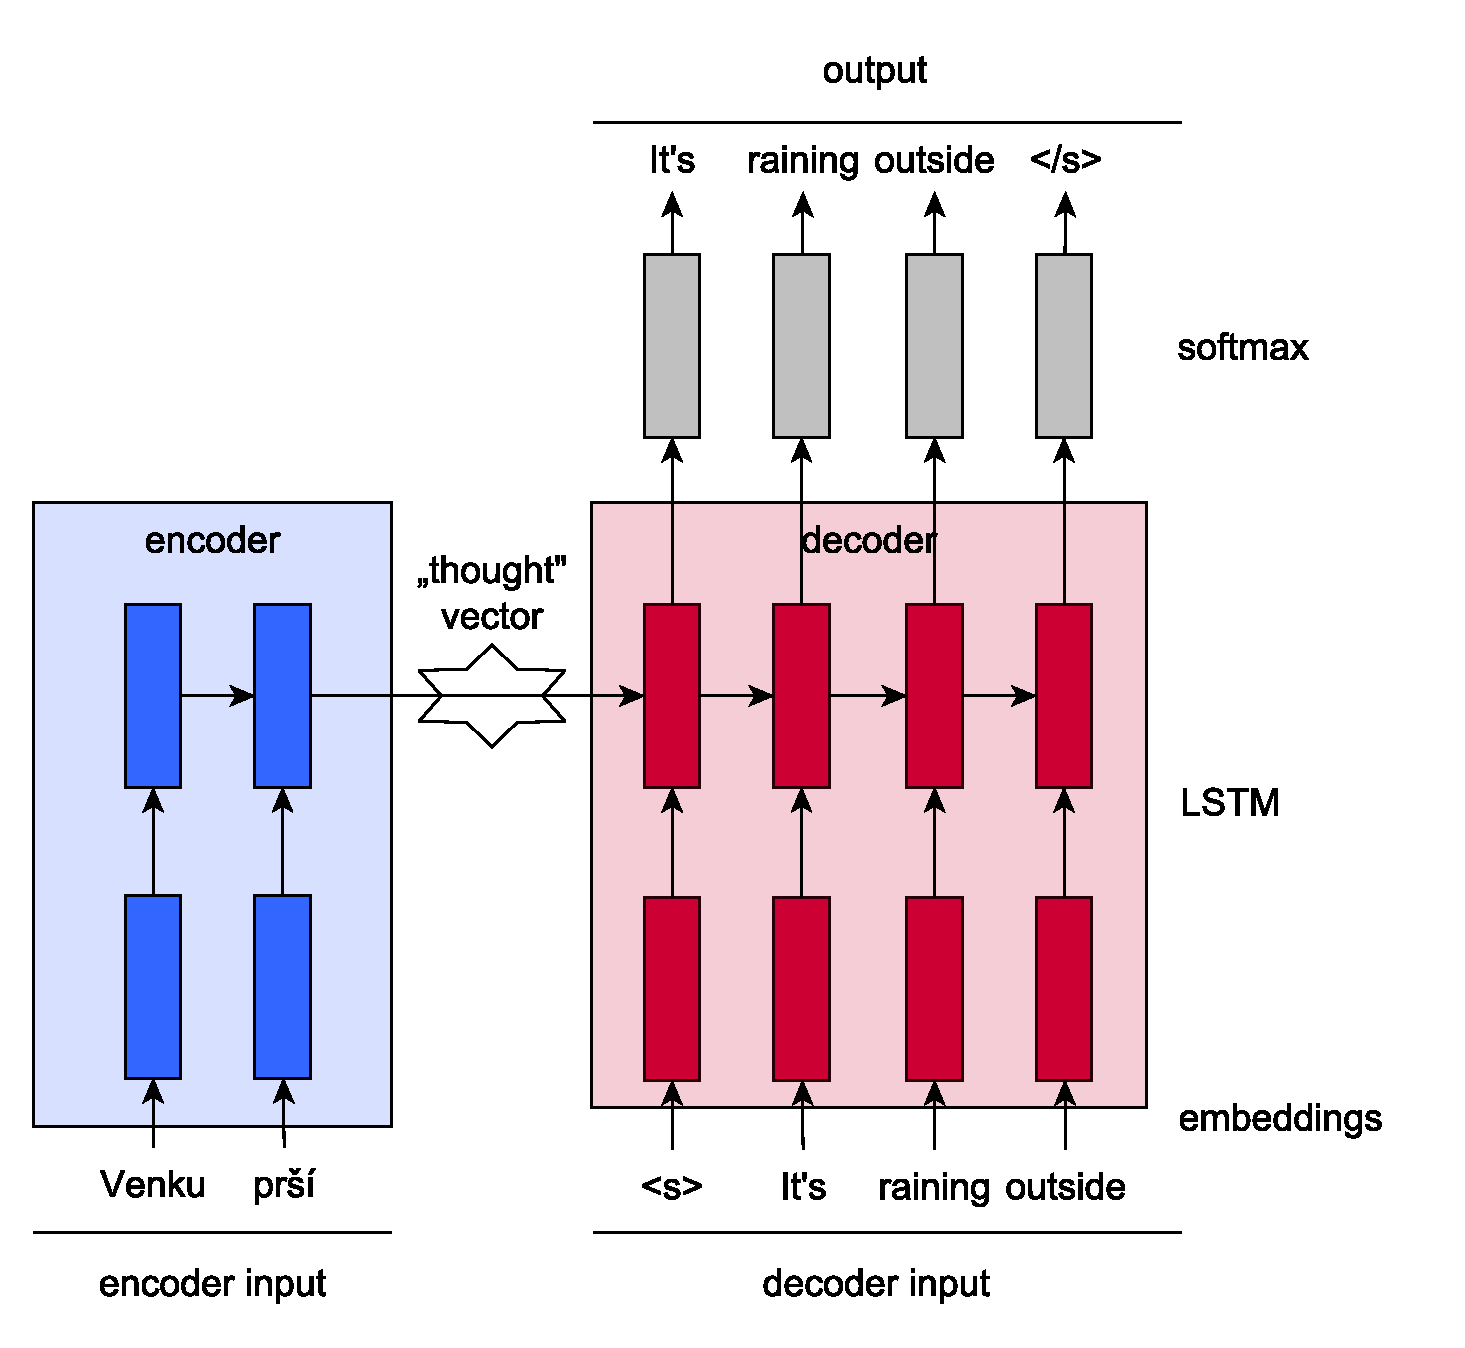
\includegraphics[width=0.75\linewidth]{seq2seqEn.pdf}\\[1pt]
  \caption{The encoder-decoder architecture shown on translation from a Czech sentence to its English equivalent. The encoder processes embeddings of the input sequence and produces the fixed-length ``thought" vector. This vector is used as initial state of the decoder, it tells it from what context should it produce the output in the target language. The prediction is started with the $\langle s \rangle$ starting token. Then the decoder is fed either correct output tokens during the training time or its own output, from the time $t - 1$, during inference time, until it generates the ending $\langle /s \rangle$ token.}
  \label{fig:seq2seq}
\end{figure*}

\hfill \break
Equations of the encoder-decoder architecture:
\begin{linenomath}
\begin{align}
    m^{(f)}_{t}&=M^{(f)}_{f_t}\label{figure:encoderEmb} \\
    h^{f}_{t}&=\begin{cases}
                    RNN^{(f)}(m^{(f)}_{t},h^{(f)}_{t-1}) & \mbox{if t $\geq$ 1},\label{figure:encoderState} \\
                    0 & \mbox{otherwise}.
                \end{cases}\\
    m^{(e)}_{t}&=M^{(e)}_{e_{t-1}}\label{figure:decoderEmb} \\
    h^{e}_{t}&=\begin{cases}
                    RNN^{(e)}(m^{(e)}_{t},h^{(e)}_{t-1}) & \mbox{if t $\geq$ 1},\\
                    h^{f}_{|F|} & \mbox{otherwise}.
                \end{cases}\label{figure:decoderState} \\
    p^{(e)}_{t}&=\mbox{softmax}(W_{hs}h^{(e)}_{t} + b_{s}) \label{figure:resultSoftmax}
\end{align}
\end{linenomath}

\begin{itemize}
    \item $RNN^{(f)}$ - encoder, $RNN^{(e)}$ - decoder
    \item $M^{(f)}_{f_t}$ - embedding for encoder input in time $t$
    \item $M^{(e)}_{e_t}$ - embedding for decoder input in time $t$
    \item $h^{(f)}_t$ - encoder hidden state in time $t$
    \item $h^{(e)}_t$ - decoder hidden state in time $t$
    \item $W_{hs}$ - weights
    \item $b_s$ - bias
\end{itemize}


An embedding is looked up for every word in time~$t$ (Eq. \ref{figure:encoderEmb}). Then the hidden state of the encoder is computed (Eq. \ref{figure:encoderState}). After processing of the whole input sequence, there should be enough context stored for the decoder initialisation. Then, as similar to the encoder, an embedding is looked up for the decoder input (Eq. \ref{figure:decoderEmb}). Only now the word is from the time $t - 1$ as the decoder generates a new word based on the last one. In the time $t_0$ the decoder is fed the starting symbol $\langle s \rangle$. Eq. \ref{figure:decoderState} computes the hidden state of the decoder and shows that in the time $t_0$, the decoder is initialised with the encoder final state. The final output probability is computed with the $softmax$ function (Eq. \ref{figure:resultSoftmax}).

An in depth overview of NMT is given in \cite{nmtTutorial}.

\section{Implementation of the NMT system}
The presented system is implemented in Python with Keras library using Tensorflow backend. The result is a python package \emph{nmt}, published on github\footnote{\url{https://github.com/jojkos/neural-machine-translation}}.

\subsection{Data preprocessing}
Some of the Moses scripts are used for preprocessing of the data. To tokenize sequences, \emph{tokenizer.perl} is used. To select proper uppercase first letter for each token, \emph{truecase.perl} is used. Cleaning is done with \emph{clean-corpus-n.perl} so that only sequences with max length of 15 tokens are kept in the dataset. To split tokens into sub-word units, \emph{subword-nmt}\footnote{\url{https://github.com/rsennrich/subword-nmt}} scripts are used.

\subsection{Implementation details}
Size of a source and a target vocabulary is clipped to a maximum size chosen in an experiment and unknown words are replaced with $\langle unk \rangle$ token. The package can be used with pre-trained word embeddings in \emph{fastText}\cite{fasttext} format. To enhance performance, bi-directional encoder is implemented, it is possible to use multiple layers for both the decoder and the encoder and during training, dropout can be specified and teacher forcing is used. LSTM is used as an RNN unit in both the encoder and the decoder. During translation generation, beam search is used to find best hypothesis with maximum score.


\section{Experiments and results}
This sections presents results of experiments conducted with the \emph{nmt} package compared with results made with baseline system created with the Moses tool. The evaluation is done with the standard BLEU metric. BLEU (\cite{BLEU}) is an algorithm for automatic evaluation of translation systems. It compares translated sentences with a~reference translations. Those scores are averaged over the whole dataset and the output is a number between 0--100, indicating how similar is the candidate text to the reference texts, the higher the more similar.

Datasets are taken from the yearly conference on machine translation (\emph{WMT} -- formerly \textbf{w}orkshop on statistical \textbf{m}achine \textbf{t}ranslation) conference. In particular, datasets from WMT17\footnote{\url{http://data.statmt.org/wmt17/translation-task/preprocessed/}} are used. They contain text data from different domains like subtitles, books, news and websites. Size of each dataset is shown in Table \ref{table:datasetsSize}.

For all experiments, pre-trained word embeddings with size of 300 dimensions were used, obtained from facebookresearch\footnote{\url{https://github.com/facebookresearch/fastText/blob/master/pretrained-vectors.md}}.

Experiments ran on VUT FIT computational cluster\footnote{\url{http://www.fit.vutbr.cz/CVT/cluster/}} on GPU. RMSprop was used as optimizer with learning rate 0.001. Each experiment ran until the result of loss function for validation dataset did not decrease for 5 epochs.

\vspace{3mm}

\begin{table}[h!]
	\caption{Examples of translations.}
	\label{table:originalExamples}
    \begin{center}
        \begin{tabular}{p{1\linewidth}}
          \toprule
          \multicolumn{1}{c}{original sentences} \\
          \midrule
          1. budoucnost se jevila černě. \\
          2. někdo mu musí dát lekci. \\
          3. nejdůležitější výsledky studie jsou uvedeny v tabulce 4 a na obrázku 3. \\
          4. uvidíme, jak se ta schůze bude odvíjet. \\
          5. Evropská unie je druhým největším obchodním partnerem ASEAN. \\
          6. 13. prosinec \\
          \bottomrule
        \end{tabular}
    \end{center}
    \begin{center}
        \begin{tabular}{p{1\linewidth}}
          \toprule
          \multicolumn{1}{c}{reference translation} \\
          \midrule
          1. the future was grey. \\
          2. somebody's got to teach him a lesson. \\
          3. the key results of the trial are listed in Table 4 and Figure 3. \\
          4. see how the meeting goes. \\
          5. the European Union is ASEAN' s second largest trading partner. \\
          6. December 13 \\
          \bottomrule
        \end{tabular}
    \end{center}
    \begin{center}
        \begin{tabular}{p{1\linewidth}}
          \toprule
          \multicolumn{1}{c}{baseline Moses system translation} \\
          \midrule
          1. the jevila black.  \\
          2. someone must give him a lesson.  \\
          3. the study results are provided in Table 4 and the picture 3. \\
          4. we'll see how the meeting is odvíjet. \\
          5.~the European Union's second largest partner ASEAN. \\
          6. 13 December \\
          \bottomrule
        \end{tabular}
    \end{center}
    \begin{center}
        \begin{tabular}{p{1\linewidth}}
          \toprule
          \multicolumn{1}{c}{presented system translation} \\
          \midrule
          1. the future was red. \\
          2. someone needs to give him a lesson. \\
          3. the most important results of the two and two are available in the level of the 3. \\
          4. let's see how the meeting goes. \\
          5. the European Agreement is the most attractive partner of the European Union. \\
          6. 13. \\
          \bottomrule
        \end{tabular}
    \end{center}
\end{table}

\begin{table}[h!]
    \caption{Number of sentence pairs for different used datasets.}
	\label{table:datasetsSize}
    \begin{center}    	
        \begin{tabular}{ll}
          \toprule
          dataset & sentence pairs \\
          \midrule
          training $Cs\rightarrow En$ & 1000000 \\
          validation $Cs\rightarrow En$ & 2000 \\
          test $Cs\rightarrow En$ & 2000 \\
          training $Cs\rightarrow En$ + $En\rightarrow De$ & 2000000 \\
          test $En\rightarrow De$ & 2000 \\
          test $Cs\rightarrow De$ & 2000 \\
          \bottomrule
        \end{tabular}
    \end{center}
\end{table}


First, several experiments with different hyperparameters were conducted on language pair Cs$\rightarrow$En, to find out optimal hyperparameters for the system. The same training dataset was used to train baseline system with Moses tool. Best performing NMT model was with hyperparameters: 2 layers LSTM of size 1000 layers for encoder, 2 LSTM of size 1000 for decoder, 15000 maximum vocabulary size, dropout of 0.1, and beam size 15. Best performing model and baseline system were evaluated with test dataset. Results are in the Table \ref{table:results} and examples of translations are in the Table \ref{table:originalExamples}.

\vspace{3mm}

\begin{table}[h!]
    \caption{Resulting BLEU score on the $Cs\rightarrow En$ test dataset of the baseline system and of the best performing model created with \emph{nmt} package. The system made with Moses tool is showing better performance.}
	\label{table:results}
    \begin{center}    	
        \begin{tabular}{ll}
          \toprule
          system & BLEU score \\
          \midrule
          baseline & 23.08  \\
          created  & 9.87 \\
          \bottomrule
        \end{tabular}
    \end{center}
\end{table}

Another experiment was conducted to find out how the performance of the model will be affected when its trained to translate on more language pairs. Training dataset included $Cs\rightarrow En$ training dataset used in previous experiments, plus another 1000000 sentence pairs for $En\rightarrow De$ pair. Model was then tested with test datasets for $Cs\rightarrow En$ pair, $En\rightarrow De$ pair and for $Cs\rightarrow De$ to try out zero-shot translation on a language pair that the model was not explicitly trained on. Results are shown in Table \ref{table:resultsMulti}.

\begin{table}[h!]
	\caption{Resulting BLEU score for different test datasets, each for one language pair. Translation was done by one model trained on multiple language pairs. Results shows, that the model is now capable to translate $Cs\rightarrow En$ and $En\rightarrow De$ for the price of having worse results for the former. Zero-shot translation for $Cs\rightarrow De$ does not show much success.}
	\label{table:resultsMulti}
    \begin{center}
        \begin{tabular}{ll}
          \toprule
          language pair & BLEU score \\
          \midrule
          $Cs\rightarrow En$ & 7.10 \\
          $En\rightarrow De$ & 7.39 \\
          $Cs\rightarrow De$ & 0.14 \\
          \bottomrule
        \end{tabular}
    \end{center}
\end{table}

Results shows that models created with the published system are capable of learning to translate between two languages and even between multiple language pairs with at least some precision. Farther investigation is needed to find out why the performance does not reach the performance of the current state-of-the-art systems and of the baseline system.

\section{Conclusions}\label{sec:Conclusions}

The goal of this paper was to explore neural machine translation and to develop a translation system with the encoder-decoder architecture. This system was built, published on github and tested against Moses statistical translation tool.

The best BLEU score on $Cs\rightarrow En$ translation of the created system is \textbf{9.87} while the system built with Moses has score \textbf{23.08}. When the system was trained on multiple languages, score for $Cs\rightarrow En$ pair dropped to \textbf{7.10} but the same model was able to translate even for $En\rightarrow De$ pair with score \textbf{7.39}. Experiment with zero-shot was not very successful and would probably require bigger training dataset. Although presented system does not give excellent results, it shows that the core is working.

Next plan is to find the reason of the subpar results and improve them. Another step would be to add attention module.

\section*{Acknowledgements}
I would like to thank my supervisor Ing. Igor Szőke, Ph.D. for his guidance.


%--------------------------------------------------------
%	REFERENCE LIST
%--------------------------------------------------------
\phantomsection
\bibliographystyle{unsrt}
\bibliography{2018-ExcelFIT-NeuralMachineTranslation}

%--------------------------------------------------------
%--------------------------------------------------------
%--------------------------------------------------------
\end{document} 